\section{Background and Motivating Example}
\label{sec:motivation}

We encountered the uncertainty problem while testing the protocol implementation
of a popular wireless game controller. A custom wireless communication protocol
was designed to meet the low latency and low power consumption goals. As is
common industry practice, the protocol specification was then handed over to
wireless chipset vendors for implementation. However, neither implementation
details nor trace collection capabilities are provided in the shipped firmware
due to intellectual property constraints and device resource limitation. Hence
using sniffers to validate the protocol implementation is the only option.

We initially developed a tool to validate certain protocol properties over the
sniffer trace, yet often found unacceptable amount of false alarms due to
the incompleteness of the sniffer traces, making the tool virtually useless. It
was clear that we needed to account for sniffer uncertainty.

To better understand the incompleteness of sniffer trace, consider the IEEE
802.11 (also known as \wifi{}) transmitter (DUT) state machine shown in
Fig.~\ref{fig:dot11_tx_ta}. After the DUT sends $DATA_i$---a data packet with
sequence number $i$ ($s_0\rightarrow s_1)$, it starts a timer and waits for the
acknowledgment packet---$Ack$. The DUT either receives $Ack$ within time $T_o$
($s_1\rightarrow s_0$), or it sends $DATA'_i$---retransmission of $DATA_i$
($s_1\rightarrow s_2$). Similarly, the DUT either receives the $Ack$ within $T_o$
($s_2\rightarrow s_0$) or aborts transmission and moves on to next
packet\footnote{To represent the state machine succinctly, our example assumes
that the DUT retries at most once.} ($s_2\rightarrow s_1$).

\begin{figure}[H]
  \centering
  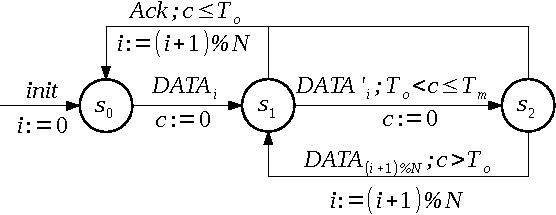
\includegraphics[width=0.6\textwidth]{./figures/dot11_tx_ta.pdf}
  \caption{\textbf{Monitor State Machine for 802.11 Transmitter.}}
  \label{fig:dot11_tx_ta}
  \vspace*{-5mm}
\end{figure}

Given a complete log of DUT's packet transmission and reception events, it is
trivial to feed such a log into the state machine in Fig.~\ref{fig:dot11_tx_ta}
and validate the correctness of DUT's protocol implementation. However, due to
DUT limitations we have described earlier, this complete log is not
available. As a result, we seek to validate the DUT implementation using
sniffers.

There are two fundamental properties in wireless communication that bring uncertainty to
sniffer's observation: packet loss and physical diversity. The sniffer could
either miss packets sent from or to the DUT due to packet loss, or overhear packets
that are sent to but missed by the DUT due to physical diversity.

\begin{figure}[H]
  \vspace*{-3mm}
  \centering
  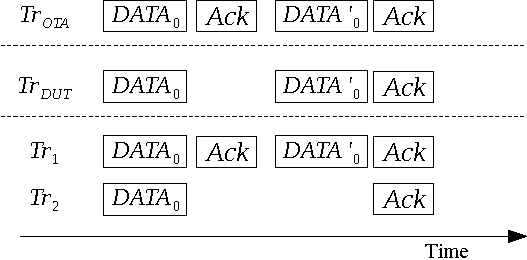
\includegraphics[width=0.6\textwidth]{./figures/false_pos.pdf}
  \caption{\textbf{Uncertainty of Sniffer Observations.} $Tr_{OTA}$ is
    the chronological sequence of packets sent by the DUT and the receiver.
    $Tr_{DUT}$ is DUT's internal events. $Tr_1$ and $Tr_2$ are two examples of
    many possible sniffer traces.}
  \label{fig:sniffer_in_middle}
  \vspace*{-5mm}
\end{figure}

Consider a correct packet exchange sequence shown in
Fig.~\ref{fig:sniffer_in_middle}. The DUT first sends $DATA_0$.  Suppose the
receiver receives $DATA_0$ and sends the $Ack$ which the DUT does not receive.
Eventually the DUT's timer fires and it sends $DATA'_0$.  This time the
$DATA'_0$ reaches receiver and the DUT also receives the $Ack$.

Now consider two possible traces that could have been overheard by a sniffer shown
in Fig.~\ref{fig:sniffer_in_middle}.
In first sniffer trace $Tr_1$ where the sniffer
\textit{overhears} the first $Ack$ packet, a validation \textit{uncertainty}
arises when the sniffer sees the $DATA'_0$: was the previous $Ack$ missed by the
DUT or is there a bug in DUT which causes it to retransmit even after receiving
the $Ack$?

Similarly, consider the second possible sniffer trace $Tr_2$
where both the $DATA'_0$ and $Ack$ packets were missed by the sniffer. During
this period of time, it appears the DUT neither receives $Ack$ for $DATA_0$ nor
sends $DATA'_0$. Again, without any additional information it is impossible to
disambiguate between the sniffer missing certain packets and a bug in DUT's
retransmission logic.

Informally, the question we set out to answer in this paper is: given the
protocol monitor state machine and the sniffer's observation with inherent
uncertainty, how to accurately validate that the DUT behaves as specified?
